\section{Introduction}

Benchmarks built from real GitHub issues have become a standard to evaluate coding agents. SWE-bench \citep{jimenez2024swebench} asks an agent to resolve an issue in a real repository and grades the resulting patch with the tests of the original fix. After frontier systems saturated its human-screened subset, SWE-bench Verified \citep{openai2024verified}, and contamination of its older issues became difficult to rule out (it could no longer be used to measure frontier capability as described in \citet{openai2026swebenchverified}). SWE-Bench Pro \citep{deng2025swebenchpro} was designed as its successor. Its public split contains 731 tasks from 11 actively maintained repositories in Python, Go and JavaScript/TypeScript. Reference solutions often span several files, and each task pairs a human-written specification (problem statement, requirements and interface) with hidden tests. SWE-Bench Pro scores are widely reported in model releases and leaderboards, and practitioners use them to select models and agent scaffolds, so keeping the benchmark accurate over time is crucial.

As agents improve, a growing share of their remaining failures traces back to issues in the tasks \citep{nadgir2026life}. We reviewed all 731 public tasks and found two classes of issues. \emph{Data defects} make a task's grade disagree with the correctness of the solution: tests that check behavior the instruction never states, instructions that contradict or leak the tests, weak tests, and verifier or environment defects (Table~\ref{tab:repairs-discards}); repairing or retiring them touched 480 tasks (66\%). \emph{Evaluation exploits} let an agent pass by cheating, without solving the task.


We address both classes of issues and release SWE-Bench Pro V2. Two agentic audits flag 200 of the 731 tasks, 23 expert software engineers adjudicate every flag, and the verifiers are hardened for all tasks (Figure~\ref{fig:pipeline}). The release has 642 tasks, 391 repaired and 89 discarded.

On V2, Claude Opus 5 (run in Claude Code) resolves 99\% of the tasks, whereas Gemini~3.8 Flash resolves 94.9\% and Inkling 89.9\% (Figure~\ref{fig:spread}). The full set still separates systems below the frontier, and a 51-task Hard split spreads systems from 52.9\% to 98.0\%.  Our contributions are:
\begin{itemize}\setlength\itemsep{0pt}
\item \textbf{SWE-Bench Pro V2}: A cleaned set of 642 tasks and an accompanying 51-task Hard split, after several rounds of automatic and expert repair: 23 engineers adjudicate every agentic audit flag (over 404 hours), validated each repair by blind re-implementation, and hardened and gated every verifier (\S\ref{sec:method}).

\item \textbf{A repair pipeline and defect taxonomy} for issue-based coding benchmarks, with agentic audits as triage, engineer adjudication, blind re-implementation and verifier hardening (\S\ref{sec:audits}--\ref{sec:verifier}).

\item \textbf{Evidence from operating the benchmark}: the exploits that in-sandbox grading admits and the locked protocol rejects (\S\ref{sec:protocol-results}), a study showing the agent harness changes cost but not accuracy for open-weight models (\S\ref{sec:harness}), and why a benchmark near saturation for frontier models remains useful (\S\ref{sec:discussion}).

\end{itemize}

%We address both classes of issues and release the result as SWE-Bench Pro V2 (\S\ref{sec:method}). The data pipeline has four stages. (1)~The two agentic audits flag 200 of the 731 tasks. (2)~23 software engineers adjudicate every flag against the task artifacts, spending 1{,}897 hours in total. They edit an instruction only where a flag is confirmed, never modify a hidden test to match an instruction, and discard tasks whose defect lies in the tests, verifier or image. (3)~In a quality-control stage, a second engineer who has seen neither the original task nor the reference patch implements each edited instruction, and the repair is accepted only if this implementation passes the hidden tests. High-priority flags additionally receive a second independent review. (4)~We harden the shared verifiers and require, before release, that the reference patch passes and the empty patch fails on every task. The release contains 642 tasks (531 never flagged, 66 repaired and 45 flagged but kept), and 89 tasks were discarded. For the evaluation, a locked protocol allows the agent to reach only the model endpoint, verifies this restriction before every run, and grades each patch in a fresh container. \jeff{Can we make figure 2 match this paragraph's 4 stages?}

%On V2, the strongest systems solve almost every task (Figure~\ref{fig:spread}). The three Claude systems resolve 99.1--99.4\% and are statistically tied, so the full set no longer distinguishes frontier systems, although it still distinguishes the others. Gemini~3.8 Flash resolves 94.9\% and Inkling 89.9\%. Because every task is solvable and correctly graded, these gaps can be attributed to the systems; our audit attributes only 3 of Gemini's 33 failures to residual task defects. To recover spread at the top, we release a Hard split of 51 tasks on which systems range from 25.5\% to 98.0\%. The split also separates two systems that are tied on the remaining tasks. The full set remains useful for evaluating smaller and open-weight systems, whose differences were previously confounded by a 20\% defect rate. Finally, on a never-public set, correcting instructions raises the pass rate on the corrected tasks by 16.4 points and changes the other tasks by less than one point. \jeff{I think this paragraph can also be shorter or doesn't need so much detail?}

% Our contributions are as follows:
% \begin{itemize}\setlength\itemsep{0pt}
% \item \textbf{A defect taxonomy and repair pipeline} for issue-based coding benchmarks that combines two agentic audits with engineer adjudication and blind re-implementation, applied to every public SWE-Bench Pro task (\S\ref{sec:audits}--\ref{sec:review}).
% \item \textbf{SWE-Bench Pro V2}, 642 repaired tasks with hardened verifiers, and a 51-task Hard split that separates frontier systems (\S\ref{sec:verifier}, \S\ref{sec:hard}) \jeff{this should be the main contribution at the top? a hardened benchmark with 1.5k+ expert hours of annotation, multiple rounds of review, and acting as a new standard.}
% \item \textbf{A locked evaluation protocol} that restricts the network to the model endpoint and re-grades every patch in a fresh container. Under this protocol, no run retrieved external content, and re-grading rejected every dependency forged outside the patch (\S\ref{sec:protocol}, \S\ref{sec:protocol-results}) \jeff{we might not need to mention this because it's a bit of an industry standard}.
% \item \textbf{Evidence and lessons from operating the benchmark}, including a controlled study on a never-public set showing that data repairs change scores on the repaired tasks, an analysis of the benchmark's usefulness near saturation, a study of how the agent harness changes the behaviour of strong open-weight models, and practical lessons for benchmark maintainers (\S\ref{sec:private}, \S\ref{sec:harness}, \S\ref{sec:discussion}).
% \end{itemize}
%We release the tasks, the Hard split, the harness configuration and the per-task grades of every run.\todo{Anonymized link.}

\begin{figure}[t]
\centering\footnotesize
\resizebox{\columnwidth}{!}{%
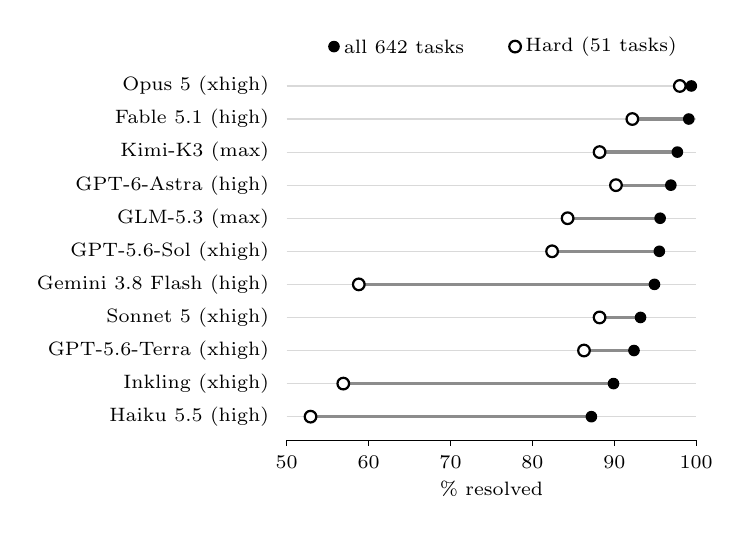
\begin{tikzpicture}
\node[anchor=east,font=\scriptsize] at (-0.1,0.00) {Opus 5 (xhigh)};
\draw[gray!30] (0,0.00) -- (5.2,0.00);
\draw[line width=1.2pt,black!45] (4.992,0.00) -- (5.138,0.00);
\fill[black] (5.138,0.00) circle (2.1pt);
\draw[black,fill=white,line width=0.8pt] (4.992,0.00) circle (2.1pt);
\node[anchor=east,font=\scriptsize] at (-0.1,-0.42) {Fable 5.1 (high)};
\draw[gray!30] (0,-0.42) -- (5.2,-0.42);
\draw[line width=1.2pt,black!45] (4.389,-0.42) -- (5.106,-0.42);
\fill[black] (5.106,-0.42) circle (2.1pt);
\draw[black,fill=white,line width=0.8pt] (4.389,-0.42) circle (2.1pt);
\node[anchor=east,font=\scriptsize] at (-0.1,-0.84) {Kimi-K3 (max)};
\draw[gray!30] (0,-0.84) -- (5.2,-0.84);
\draw[line width=1.2pt,black!45] (3.973,-0.84) -- (4.961,-0.84);
\fill[black] (4.961,-0.84) circle (2.1pt);
\draw[black,fill=white,line width=0.8pt] (3.973,-0.84) circle (2.1pt);
\node[anchor=east,font=\scriptsize] at (-0.1,-1.26) {GPT-6-Astra (high)};
\draw[gray!30] (0,-1.26) -- (5.2,-1.26);
\draw[line width=1.2pt,black!45] (4.181,-1.26) -- (4.878,-1.26);
\fill[black] (4.878,-1.26) circle (2.1pt);
\draw[black,fill=white,line width=0.8pt] (4.181,-1.26) circle (2.1pt);
\node[anchor=east,font=\scriptsize] at (-0.1,-1.68) {GLM-5.3 (max)};
\draw[gray!30] (0,-1.68) -- (5.2,-1.68);
\draw[line width=1.2pt,black!45] (3.567,-1.68) -- (4.742,-1.68);
\fill[black] (4.742,-1.68) circle (2.1pt);
\draw[black,fill=white,line width=0.8pt] (3.567,-1.68) circle (2.1pt);
\node[anchor=east,font=\scriptsize] at (-0.1,-2.10) {GPT-5.6-Sol (xhigh)};
\draw[gray!30] (0,-2.10) -- (5.2,-2.10);
\draw[line width=1.2pt,black!45] (3.370,-2.10) -- (4.732,-2.10);
\fill[black] (4.732,-2.10) circle (2.1pt);
\draw[black,fill=white,line width=0.8pt] (3.370,-2.10) circle (2.1pt);
\node[anchor=east,font=\scriptsize] at (-0.1,-2.52) {Gemini 3.8 Flash (high)};
\draw[gray!30] (0,-2.52) -- (5.2,-2.52);
\draw[line width=1.2pt,black!45] (0.915,-2.52) -- (4.670,-2.52);
\fill[black] (4.670,-2.52) circle (2.1pt);
\draw[black,fill=white,line width=0.8pt] (0.915,-2.52) circle (2.1pt);
\node[anchor=east,font=\scriptsize] at (-0.1,-2.94) {Sonnet 5 (xhigh)};
\draw[gray!30] (0,-2.94) -- (5.2,-2.94);
\draw[line width=1.2pt,black!45] (3.973,-2.94) -- (4.493,-2.94);
\fill[black] (4.493,-2.94) circle (2.1pt);
\draw[black,fill=white,line width=0.8pt] (3.973,-2.94) circle (2.1pt);
\node[anchor=east,font=\scriptsize] at (-0.1,-3.36) {GPT-5.6-Terra (xhigh)};
\draw[gray!30] (0,-3.36) -- (5.2,-3.36);
\draw[line width=1.2pt,black!45] (3.775,-3.36) -- (4.410,-3.36);
\fill[black] (4.410,-3.36) circle (2.1pt);
\draw[black,fill=white,line width=0.8pt] (3.775,-3.36) circle (2.1pt);
\node[anchor=east,font=\scriptsize] at (-0.1,-3.78) {Inkling (xhigh)};
\draw[gray!30] (0,-3.78) -- (5.2,-3.78);
\draw[line width=1.2pt,black!45] (0.718,-3.78) -- (4.150,-3.78);
\fill[black] (4.150,-3.78) circle (2.1pt);
\draw[black,fill=white,line width=0.8pt] (0.718,-3.78) circle (2.1pt);
\node[anchor=east,font=\scriptsize] at (-0.1,-4.20) {Haiku 5.5 (high)};
\draw[gray!30] (0,-4.20) -- (5.2,-4.20);
\draw[line width=1.2pt,black!45] (0.302,-4.20) -- (3.869,-4.20);
\fill[black] (3.869,-4.20) circle (2.1pt);
\draw[black,fill=white,line width=0.8pt] (0.302,-4.20) circle (2.1pt);
\draw (0,-4.50) -- (5.2,-4.50);
\draw (0.000,-4.50) -- (0.000,-4.57) node[below,font=\scriptsize] {50};
\draw (1.040,-4.50) -- (1.040,-4.57) node[below,font=\scriptsize] {60};
\draw (2.080,-4.50) -- (2.080,-4.57) node[below,font=\scriptsize] {70};
\draw (3.120,-4.50) -- (3.120,-4.57) node[below,font=\scriptsize] {80};
\draw (4.160,-4.50) -- (4.160,-4.57) node[below,font=\scriptsize] {90};
\draw (5.200,-4.50) -- (5.200,-4.57) node[below,font=\scriptsize] {100};
\node[font=\scriptsize] at (2.60,-5.12) {\% resolved};
\fill[black] (0.6,0.5) circle (2.1pt) node[right,font=\scriptsize] {all 642 tasks};
\draw[black,fill=white,line width=0.8pt] (2.9,0.5) circle (2.1pt) node[right,font=\scriptsize] {Hard (51 tasks)};
\end{tikzpicture}}
\caption{Percent of tasks resolved on SWE-Bench Pro V2 (filled dots) and its Hard split (open dots). The full set separates these systems by about 12 points (87.2--99.4\%) while the Hard split spans from 52.9\% to 98.0\%.}
\label{fig:spread}
\end{figure}
